
% TODO: add picture of collections
% \begin{frame}[fragile]
%   \frametitle{Collections of Objects}
%   \begin{itemize}
%     \item Many problems have inherent order or structure
%     \item Especially in Computer Science and Engineering (CSE) problems
%     \item Solution should use matching abstractions
%     \item Arrays, lists, maps of parallel objects
%     \item Specific segment of data, and associated computation and
%       communication
%     \item Need system support for efficient indexing
%   \end{itemize}
% \end{frame}

\begin{frame}[fragile]
  \frametitle{Collections of Objects: Concepts}
  \begin{itemize}
    \item Objects can be grouped into indexed collections
    \item Basic examples
      \begin{itemize}
      \item Matrix block
      \item Chunk of unstructured mesh
      \item Portion of distributed data structure
      \item Volume of simulation space
      \end{itemize}
      \pause
    \item Advanced Examples
      \begin{itemize}
      \item Abstract portions of computation
      \item Interactions among basic objects or underlying entities
      \end{itemize}
  \end{itemize}
\end{frame}

\begin{frame}[fragile]
  \frametitle{Collections of Objects}
  \begin{itemize}
    \item Structured: 1D, 2D, \ldots, 6D
    \item Unstructured: Anything hashable
      \pause
    \item Dense
    \item Sparse
      \pause
    \item Static - all created at once
    \item Dynamic - elements come and go
  \end{itemize}
\end{frame}

\begin{frame}[fragile]
  \frametitle{Collections of Objects: Communication}
  \begin{itemize}
    \item Point-to-point: to one element of a collection
    \item Broadcast: message to whole collection
    \item Multicast: message to subset of collection
    \item Reductions: message from (part of) collection
    \item Runtime system provides efficient delivery for all
  \end{itemize}
\end{frame}

% \begin{frame}[fragile]
%   \frametitle{Collections of Objects: Runtime Service}
%   \begin{itemize}
%     \item System knows how to `find' objects efficiently: $(collection, index) \to processor$
%     \item Applications can specify a mapping, or use simple
%       runtime-provided options (e.g. blocked, round-robin)
%     \item Distribution can be static, or dynamic!
%     \item Key abstraction: application logic doesn't change, even
%       though performance might
%   \end{itemize}
% \end{frame}

% \begin{frame}[fragile]
%   \frametitle{Collections of Objects: Runtime Service}
%   \begin{itemize}
%     \item Can develop and test logic in objects separately from their distribution
%     \item Separation in time: make it work, then make it fast
%     \item Division of labor: domain specialist writes object code, computationalist writes mapping
%     \item Portability: different mappings for different systems, scales, or configurations
%     \item Shared progress: improved mapping techniques can benefit existing code
%   \end{itemize}
% \end{frame}

\begin{frame}[fragile]
  \frametitle{Collections of Objects}
  \begin{center}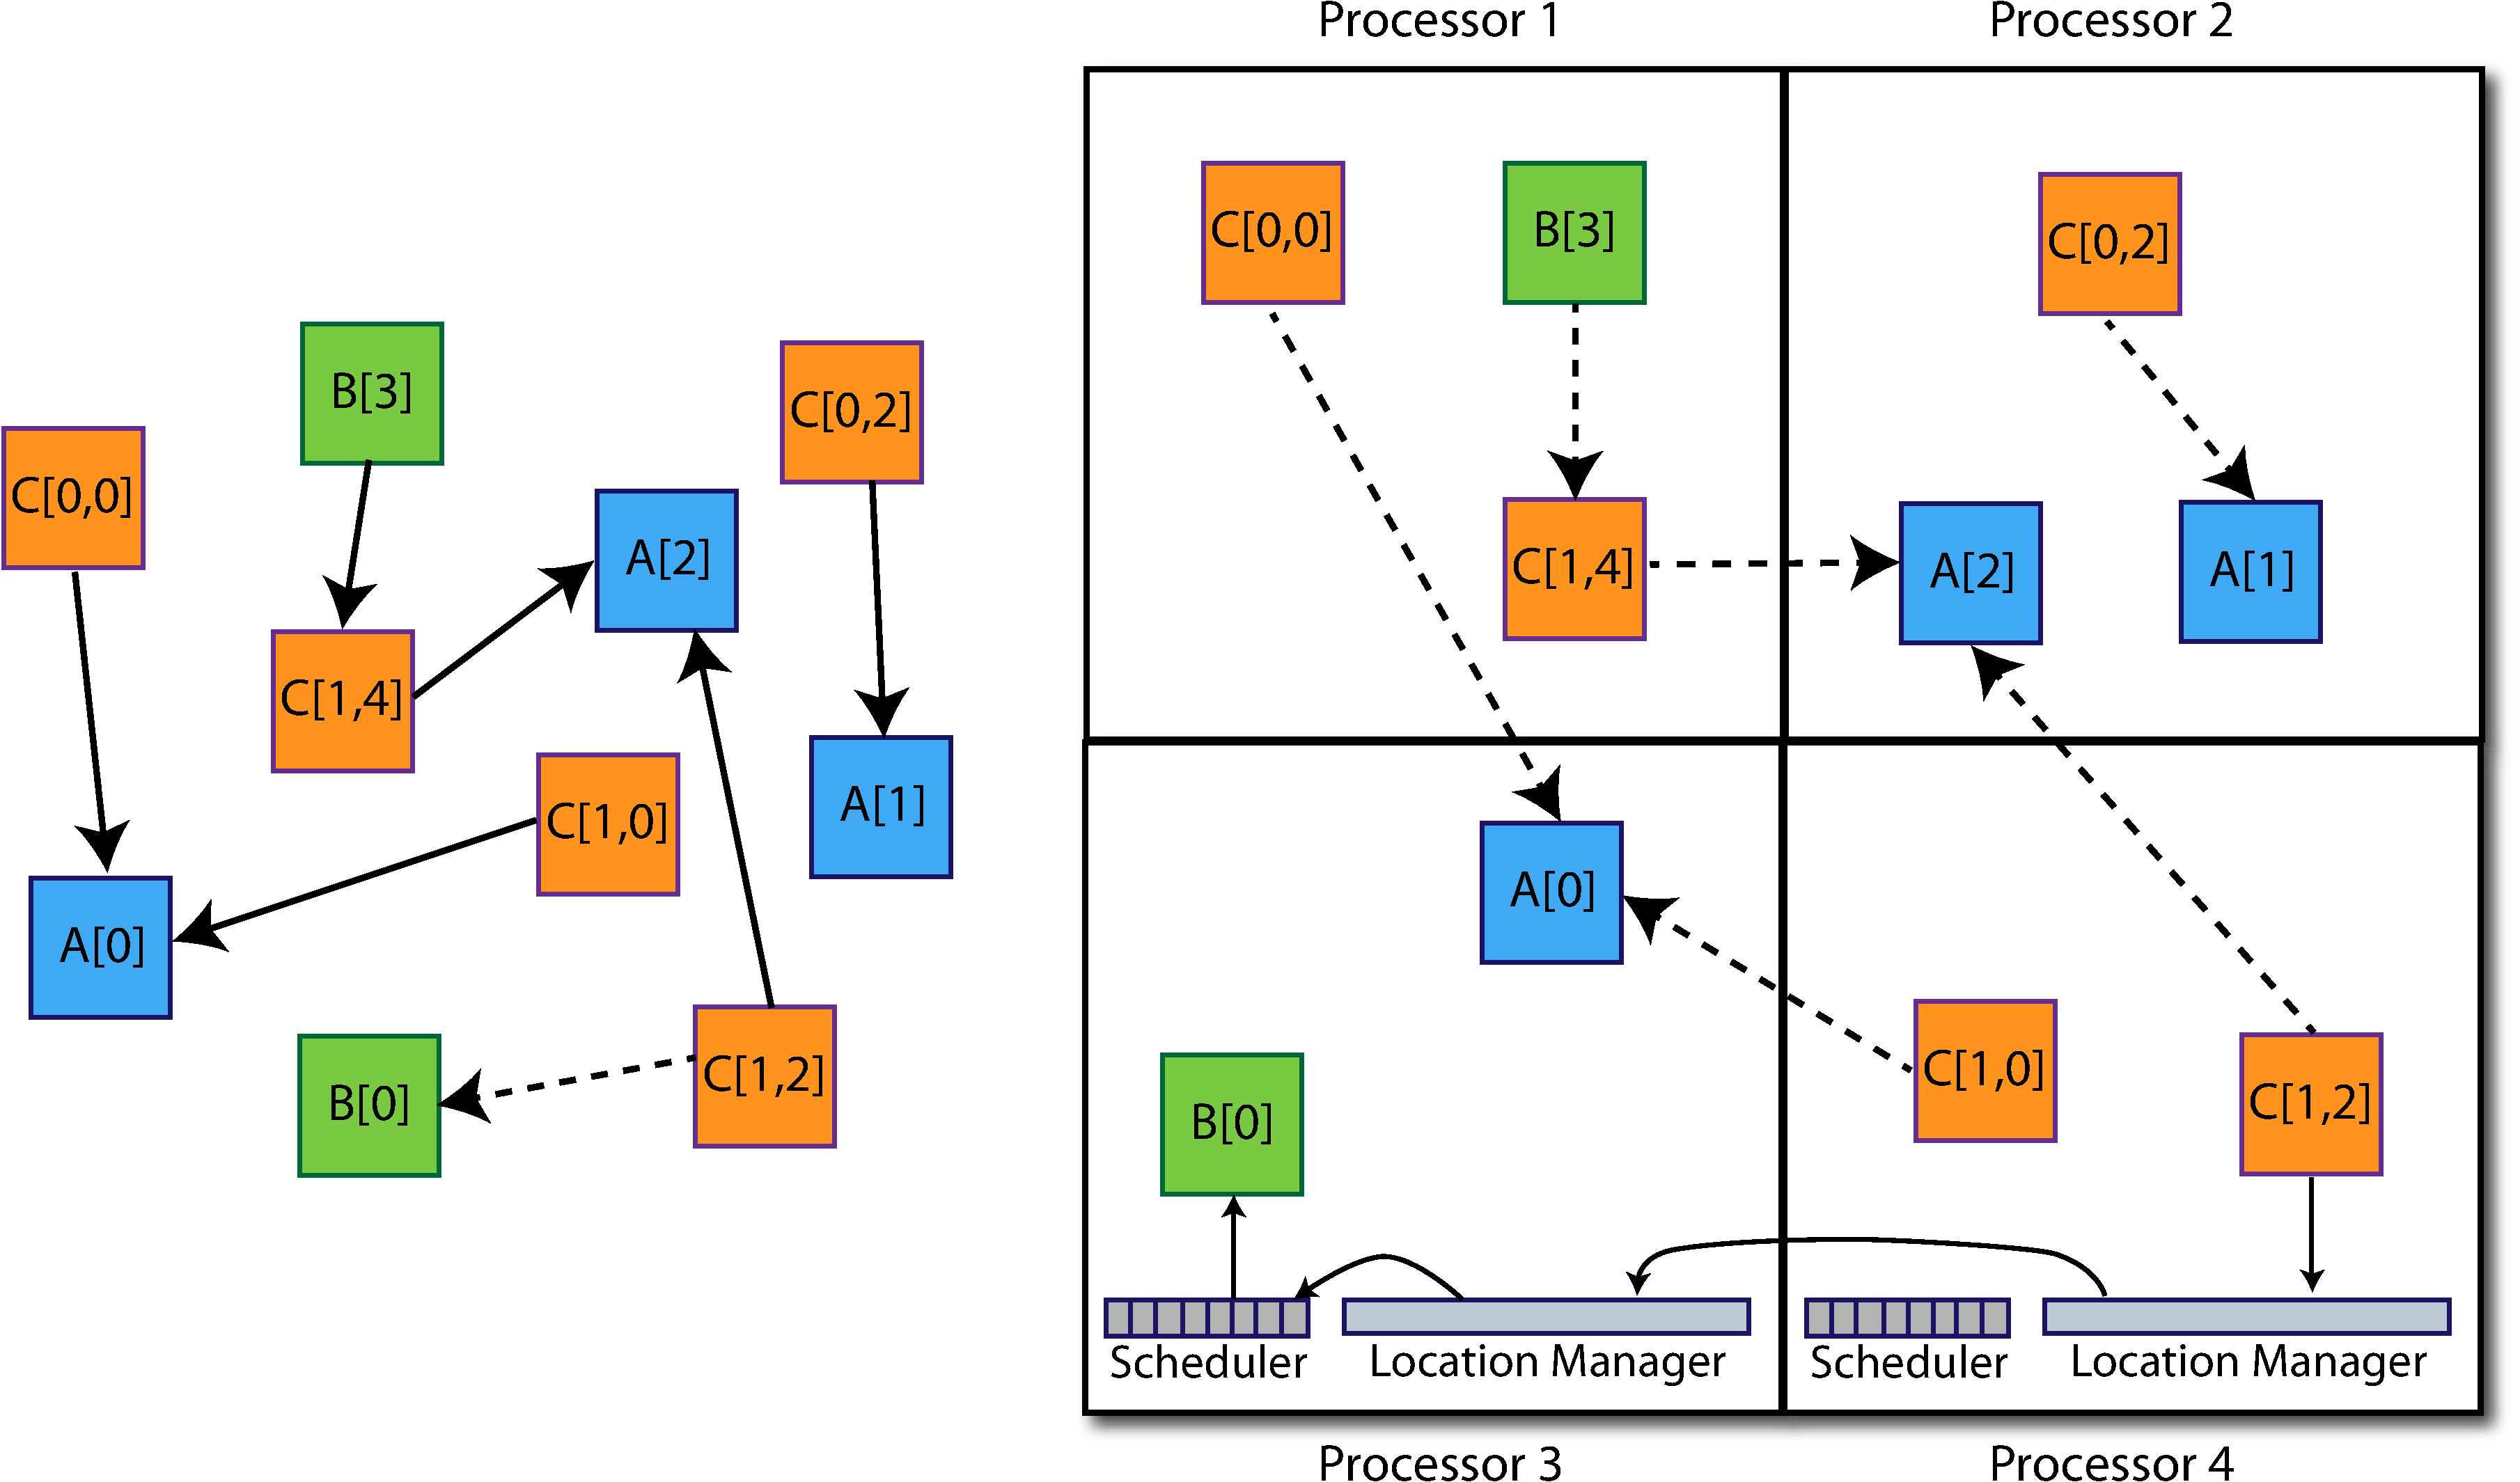
\includegraphics[width=0.9\textwidth]{figures/elements2.pdf}\end{center}
\end{frame}



%% Object Collections: Supporting Data Decomposition (Phil)

%%     Motivate why object collections are needed
%%         simple adding numbers example
%%     Object Collections
%%         decompose data and associated work
%%         1/2/3D or more (eg: mesh chunk)
%%         dense / sparse (sparse solvers, collision detection)
%%         grow / shrink dynamically (AMR)
%%         each object exposes same functionality (methods)
%%         collection should be collectively addressable (method invocation on all objects)
%%         show sample pseudo-code snippets
%%     Object Collections: Collectives
%%     Examples
%%         simple scale a distributed vector (mcast)
%%         simple add array of numbers (mcast + redn)
%%         matrix vector product (mcast + gather)
